\newpage
\section{Ομαδοποίηση}
\subsection{Εισαγωγή στην ομαδοποίηση}
Η ενότητα αυτή αφορά τους αλγορίθμους ομαδοποίησης(\textlatin{clustering}). Η δουλειά των
αλγορίθμων αυτών είναι να χωρίσουν το σύνολο των δεδομένων σε ομάδες τέτοιες ώστε τα δεδομένα μιας
ομάδας να εμφανίζουν περισσότερες ομοιότητες μεταξύ τους από ότι με τα δεδομένα των άλλων ομάδων.
Αυτός είναι και ο βασικός στόχος της διερευνητικής και στατιστικής ανάλυσης και χρησιμοποιείται
για\cite{wikicl}:
\begin{itemize}
    \item Αναγνώριση προτύπων
    \item Ανάλυση εικόνων
    \item Εξαγωγή πληροφορίας
    \item Συμπίεση δεδομένων
    \item Γραφικά υπολογιστών
    \item Μηχανική μάθηση
\end{itemize}
\begin{figure}[H]
    \centering
    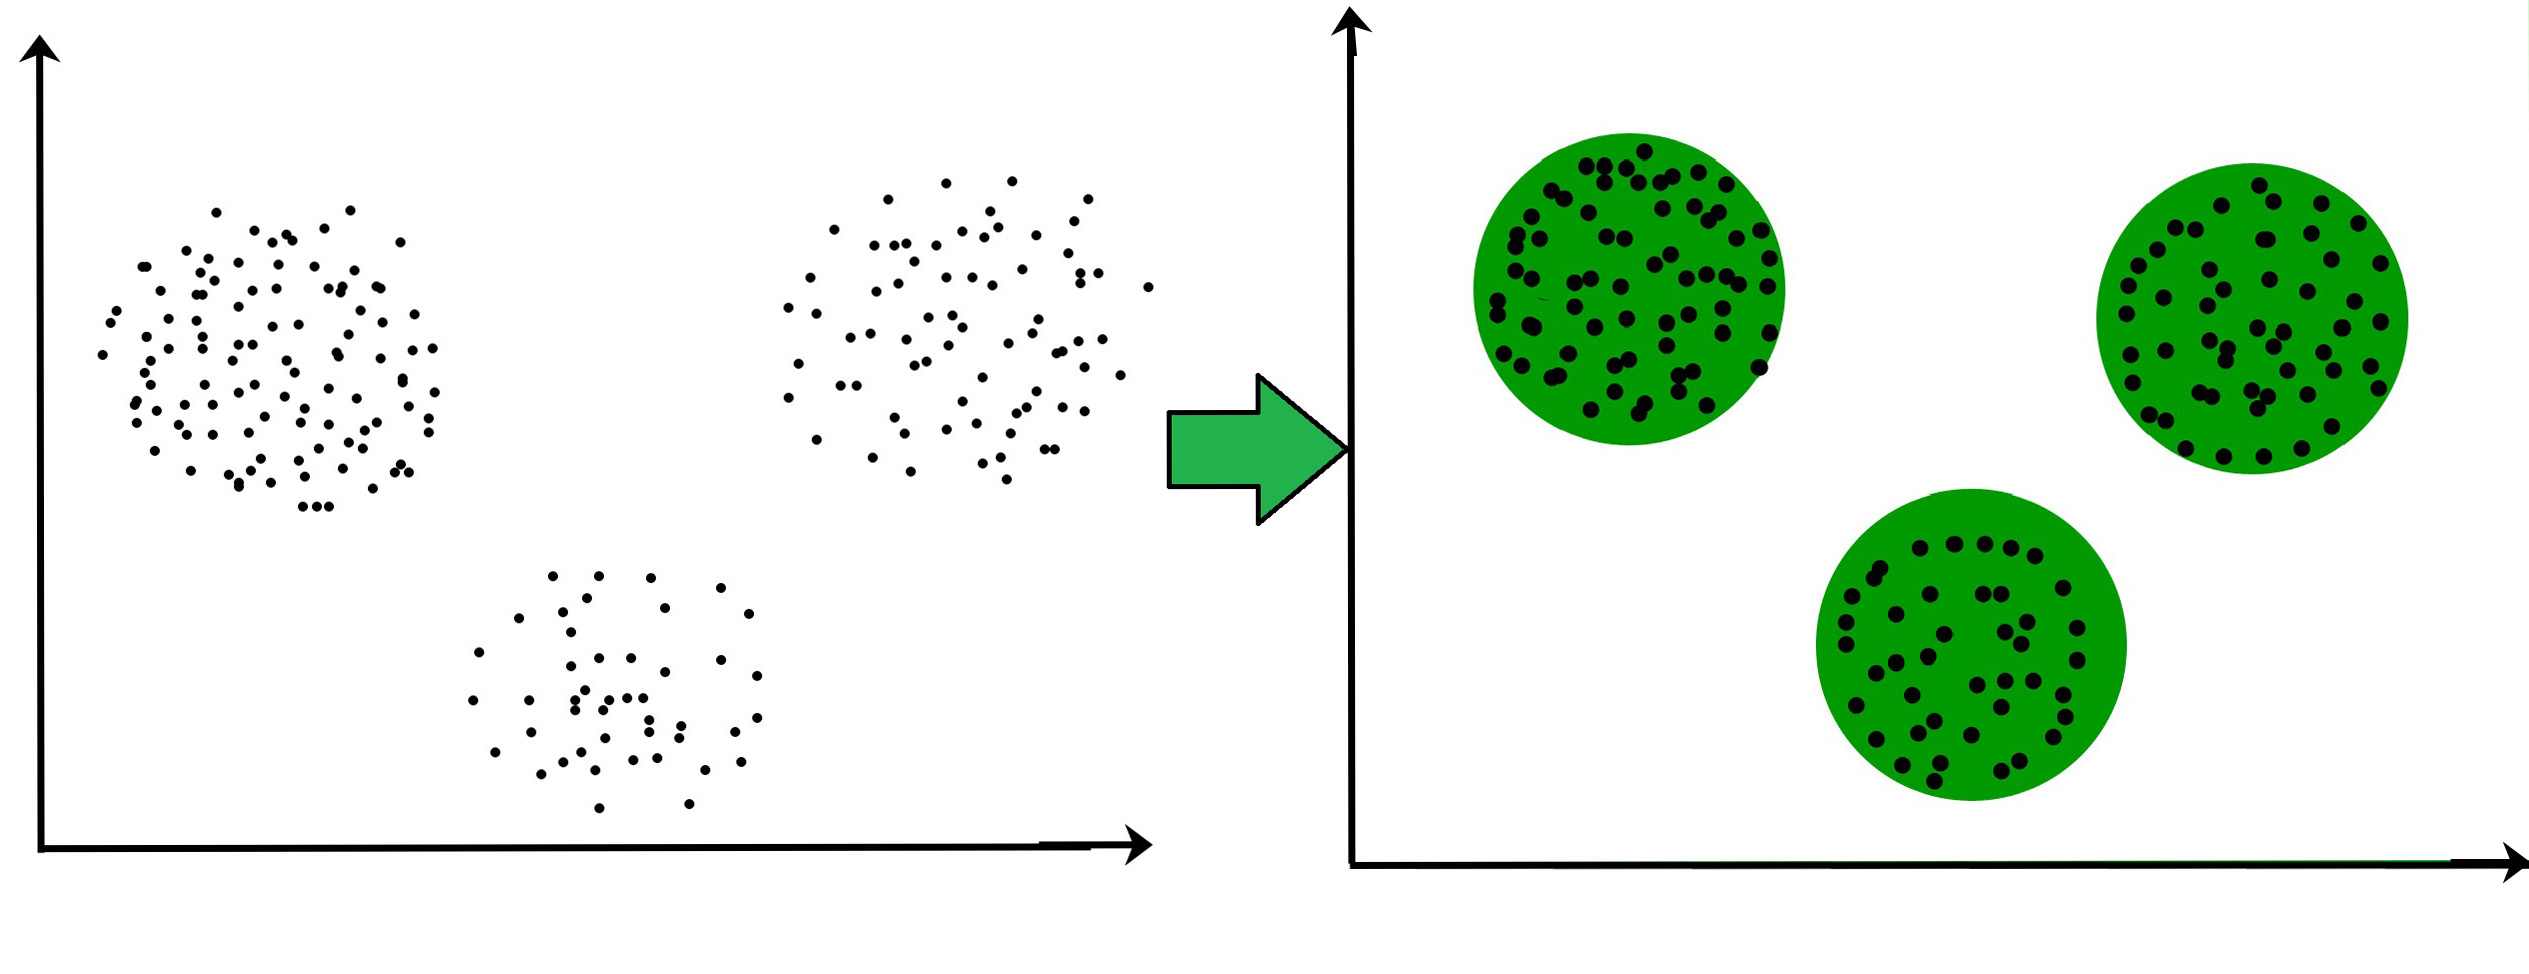
\includegraphics[width=0.7\textwidth]{images/clustering_intro.jpg}
    \caption{Γραφική αναπαράσταση ομαδοποίησης}
\end{figure}
\sloppy
Υπάρχουν εκατοντάδες αλγόριθμοι ομαδοποίησης οι οποίοι χρησιμοποιούν διαφορετικές μεθόδους και
τεχνικές. Δεν υπάρχει κάποιος που να υπερτερεί πλήρως των υπολοίπων αλλά η καταλληλότητα του Κάθε
αλγορίθμου εξαρτάται από το σύνολο δεδομένων. Παρά τις διαφορές τους μπορούμε να τους εντάξουμε σε
κατηγορίες συμφωνά με τον τρόπο που κάνουν την ομαδοποίηση. Οι τέσσερις πιο βασικές κατηγορίες
είναι:
\fussy
\begin{itemize}
    \item \textlatin{Centroid based clustering}
    \item \textlatin{Density based clustering}
    \item \textlatin{Distribution based clustering}
    \item \textlatin{Hierarchical clustering}
\end{itemize}
Οι κατηγορίες αυτές θα αναλυθούν περισσότερο στη συνέχεια. Επιπλέον, θα δούμε και τους πιο διάσημους αλγορίθμους που ανήκουν σε αυτές της κατηγορίες και θα αναλύσουμε και τον τρόπο
λειτουργίας τους.

\subsection{\textlatin{Centroid based clustering}}
Οι αλγόριθμοι τύπου \textlatin{Centroid based clustering} όπως μπορούμε να καταλάβουμε κάνουν ομαδοποίηση με βάση τα κέντρα. Αυτό σημαίνει ότι θα έχουμε τόσα κέντρα όσες και οι ομάδες που επιλέξαμε.
Έπειτα για να ομαδοποιήσουμε όλα τα σημεία του χώρου θα βλέπουμε σε ποιο κέντρο βρίσκονται πιο κοντά και θα τα εντάσσουμε στην ομάδα αυτού του κέντρου. Το πρόβλημα εδώ είναι πως θα βρούμε τα
κατάλληλα κέντρα. Αν δεν επιλέξουμε τα κέντρα σωστά τότε η ομαδοποίηση πυ θα κάνουμε θα απέχει πολύ από την πραγματικότητα. Γι' αυτό και οι συγκεκριμένοι αλγόριθμοι έχουν ως βασική δουλειά να
προσεγγίσουν αυτά τα κέντρα.\par Για να καταλάβουμε με ποιον τροπο συμβαίνει αυτό θα δούμε τον αλγόριθμο \textlatin{k-Means} που είναι και ο πιο διάσημος αλγόριθμος ταξινόμησης με βάση τα κέντρα.
Το \textlatin{k} είναι το πλήθος των ομάδων που θέλουμε. ξεκινάμε τον αλγόριθμο επιλέγοντας \textlatin{k} τυχαία κέντρα στον χώρο και χωρίζουμε τα υπόλοιπα σημεία σε ομάδες ανάλογά με την εγγύτητα
τους στα τυχαία κέντρα. Έτσι έχουμε καταλήξει σε μια αρχική προσέγγιση. Έπειτα θα βρούμε το πραγματικό κέντρο των ομάδων που δημιουργήθηκαν βρίσκοντας τη μέση τιμή των σημείων που ανήκουν στην
ομάδα. Αυτή η διαδικασία επαναλαμβάνεται και έτσι κάποια στιγμή τα τελικά κέντρα θα μπορούν να κάνουν καλή ομαδοποίηση.
\begin{figure}[H]
    \centering
    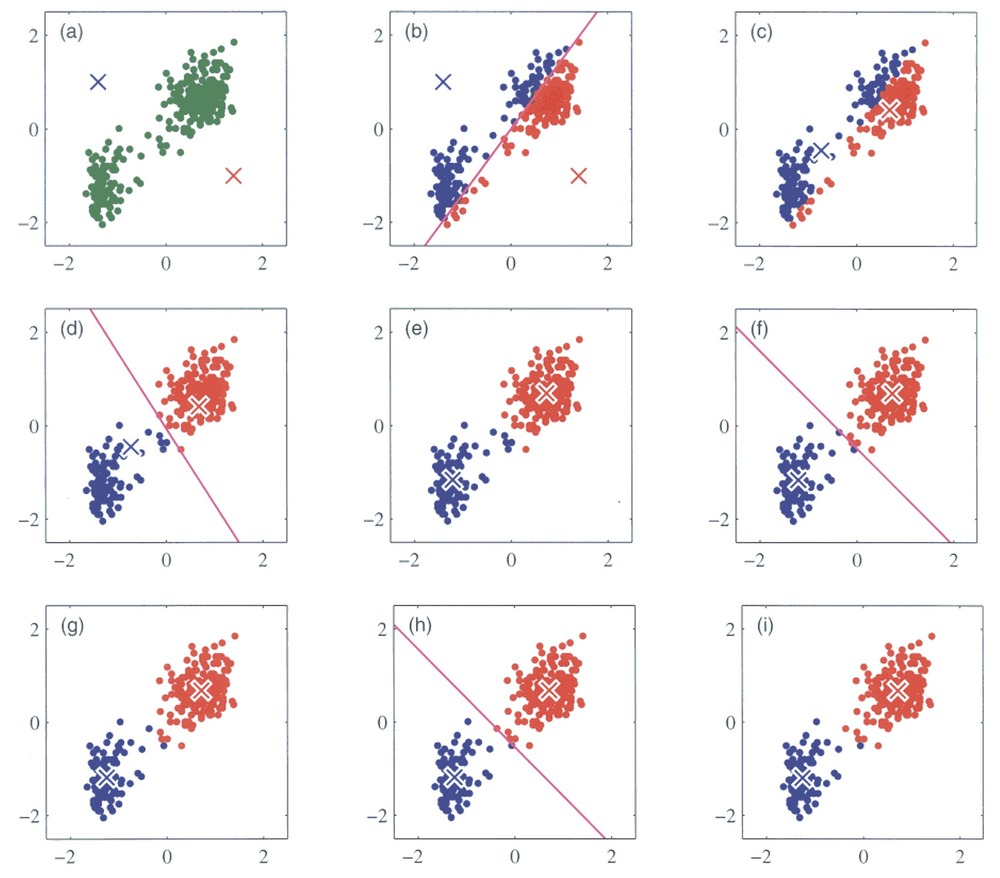
\includegraphics[width=1\textwidth]{images/kmeans.jpg}
    \caption{Επαναλήψεις του αλγορίθμου \textlatin{k-Means}}
\end{figure}
Ένα από τα πλεονεκτήματα του αλγορίθμου είναι η απλότητα του. Επιπλέον λειτουργεί καλά σε μεγάλο σύνολο δεδομένων και εξασφαλίζει ότι θα συγκλίνει σε κάποια λύση. Επίσης μπορεί αν δημιουργήσει
ομάδες διαφορετικού μεγέθους και σχήματος. Παρ' όλα αυτά τα αποτελέσματα τα τελικά αποτελέσματα του αλγορίθμου εξαρτώνται από τις αρχικές συνθηκες. Άρα εφόσον αρχικοποιούμε τα κέντρα τυχαία, αν
ξανά τρέξουμε τον αλγόριθμο θα πάρουμε διαφορετικά αποτελέσματα. Επίσης πρέπει να ορίσουμε μόνοι μας το πλήθος των ομάδων που είναι κάτι που μπορεί να μην θέλουμε πάντα\cite{kmeans1}.
\subsection{\textlatin{Density based clustering}}
Ο επόμενος τύπος αλγορίθμου που θα δούμε είναι η ομαδοποίηση με βάση την πυκνότητα. Οι συγκεκριμένοι αλγόριθμοι ανιχνεύουν τις περιοχές με μεγάλη συγκέντρωση σημείων ο ποίες διαχωρίζονται μεταξύ
τους από περιοχές που τα σημεία είναι πολύ αραιά. Αυτές οι περιοχές θα είναι και οι ομάδες που θα δημιουργηθούν και τα σημεία στις αραιές περιοχές θα θεωρηθούν θόρυβος\cite{dbclust1}.\par Ας δούμε
πως λειτουργεί ο αλγόριθμος \textlatin{DBSCAN (Density-based spatial clustering of applications with noise)} ο οποίος είναι από τους πιο διάσημους αλγορίθμους ομαδοποίησης. Για αυτόν τον αλγόριθμο
πρέπει να ορίσουμε μια παράμετρο ελάχιστης απόστασης και μία παράμετρο ελάχιστων σημείων. Έπειτα θεωρούμε τις εξής κατηγορίες σημείων:
\begin{description}
    \item[Κύρια σημεία] Έχει γειτονικά σημεία τουλάχιστον όσα τα ελάχιστα σε απόσταση μικρότερη από την ελάχιστη.
    \item[Άμεσα προσιτά σημεία] Για ένα κύριο σημείο ένα άλλο σημείο είναι προσιτό αν είναι μέσα στην ελάχιστη απόσταση.
    \item[Προσιτά σημεία] Έμα σημείο είναι προσιτό αν υπάρχει ένα μονοπάτι από σημεία που το κάθε ένα είναι άμεσα προσιτό με το διπλανό του. Το σημείο εκκίνησης πρέπει να είναι κύριο σημείο.
    \item[Θόρυβος] Όλα τα υπόλοιπα σημεία που περίσσεψαν.
\end{description}
Έπειτα κάθε κύριο σημείο δημιουργεί μία ομάδα με όλα τα προσιτά σημεία σε αυτό\cite{dbscan}.
\begin{figure}[H]
    \centering
    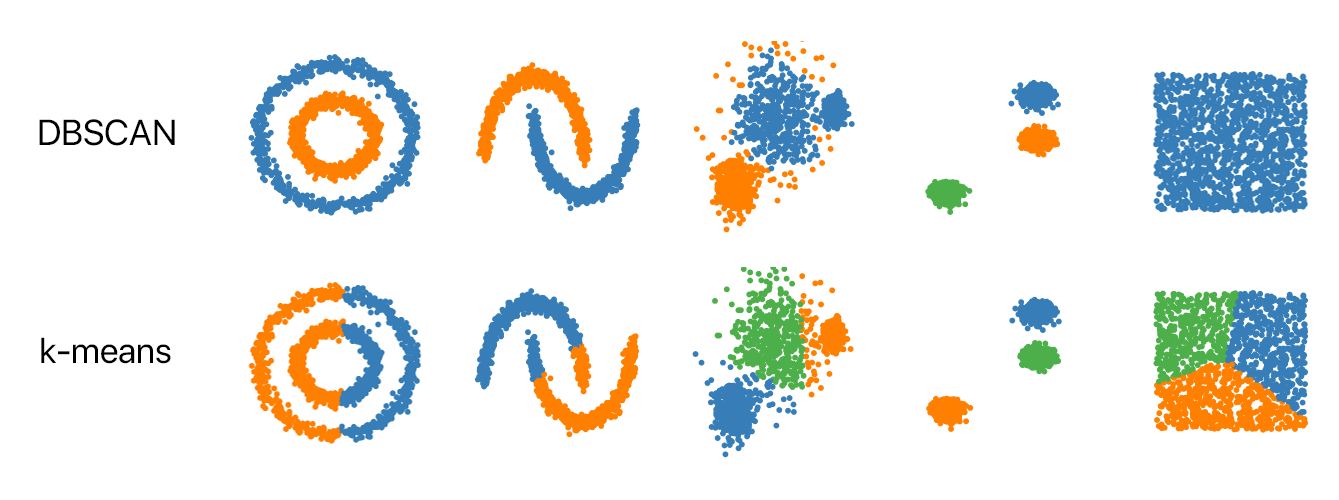
\includegraphics[width=0.8\textwidth]{images/dbscan.png}
    \caption{Αποτελέσματα ομαδοποίησης με \textlatin{DBSCAN vs k-Means}}
\end{figure}
Άπό το παραπάνω σχήμα μπορεί να καταλάβει κανείς τις περιπτώσεις που ο αλγόριθμος \textlatin{DBSCAN} υπερισχύει του \textlatin{k-Means}. Όπως φαίνεται ο \textlatin{DBSCAN} είναι κατάλληλος όταν
οι ομάδες δεν έχουν απλά σχήματα και επιπλέον μπορεί να διαλέξει μόνος του τον κατάλληλο αριθμό ομάδων που πρέπει να δημιουργήσει κάθε φορά. Συνοψίζοντας τα πλεονεκτήματα του αλγορίθμου
είναι\cite{dbscanadv}:
\begin{itemize}
    \item Δεν χρειάζεται να ορίσουμε τον αριθμό τον ομάδων
    \item Δουλεύει καλά σε ομάδες με αυθαίρετα σχήματα
    \item Μπορεί να καταλάβει ποια σημεία αποτελούν θόρυβο και να  μην τα λάβει υπόψη του
\end{itemize}
Παρ' όλα αυτά υπάρχουν και μειονεκτήματα:
\begin{itemize}
    \item Δέν μπορεί να ομαδοποιήσει δεδομένα που έχουν μεγάλες διαφορές μεταξύ τους γιατί δεν μπορούμε να επιλέξουμε τις παραμέτρους του συστήματος ώστε να ευνοούν όλες τις ομάδες
    \item Επίσης δεν μπορούμε να διαλέξουμε μια καλή τιμή για την ελάχιστη απόσταση αν δεν έχουμε καλή κατανόηση των δεδομένων
    \item Δίνει διαφορετικά αποτελέσματα κάθε φορά διότι ξεκινάει την ανάλυση από τυχαία σημεία
\end{itemize}
\subsection{\textlatin{Hierarchical clustering}}
Το \textlatin{Hierarchical clustering} είναι μια μέθοδος ομαδοποίησης η οποία προσπαθεί να δημιουργήσει μια ιεραρχία από ομάδες. Για αυτούς τους αλγόριθμους μπορούμε να διακρίνουμε δύο μεγάλες
κατηγορίες\cite{wkhc}:
\begin{description}
    \item[Συσσωματωτική] Προσεγγίζει το πρόβλημα από κάτω προς τα πάνω. Το κάθε δείγμα φτιάχνει τη δικιά του ομάδα και όταν ανεβαίνουμε στην ιεραρχία οι ομάδες αυτές συγχωνεύονται σε μεγαλύτερες
    \item[Διαιρετική] Προσεγγίζει το πρόβλημα από κάτω προς τα πάνω. Ξεκινάμε από μια μεγάλη ομάδα η οποία διαχωρίζεται σε μικρότερες αναδρομικά καθώς κατεβαίνουμε στην ιεραρχία.
\end{description}
Για να αποφασίσουμε πότε δύο ομάδες πρέπει να ενωθούν ή να διαχωριστούν πρέπει να βρούμε μια μετρική ανομοιότητας μεταξύ των σημείων. Αυτή η μετρική τις περισσότερες φορές είναι η απόσταση η οποία μπορεί να είναι η ευκλείδεια η κάποια άλλη που έχουμε ήδη αναλύσει.\par
Τα αποτελέσματα του αλγορίθμου μπορούν να αναπαρασταθούν με τη μορφή δέντρου
\begin{figure}[H]
    \centering
    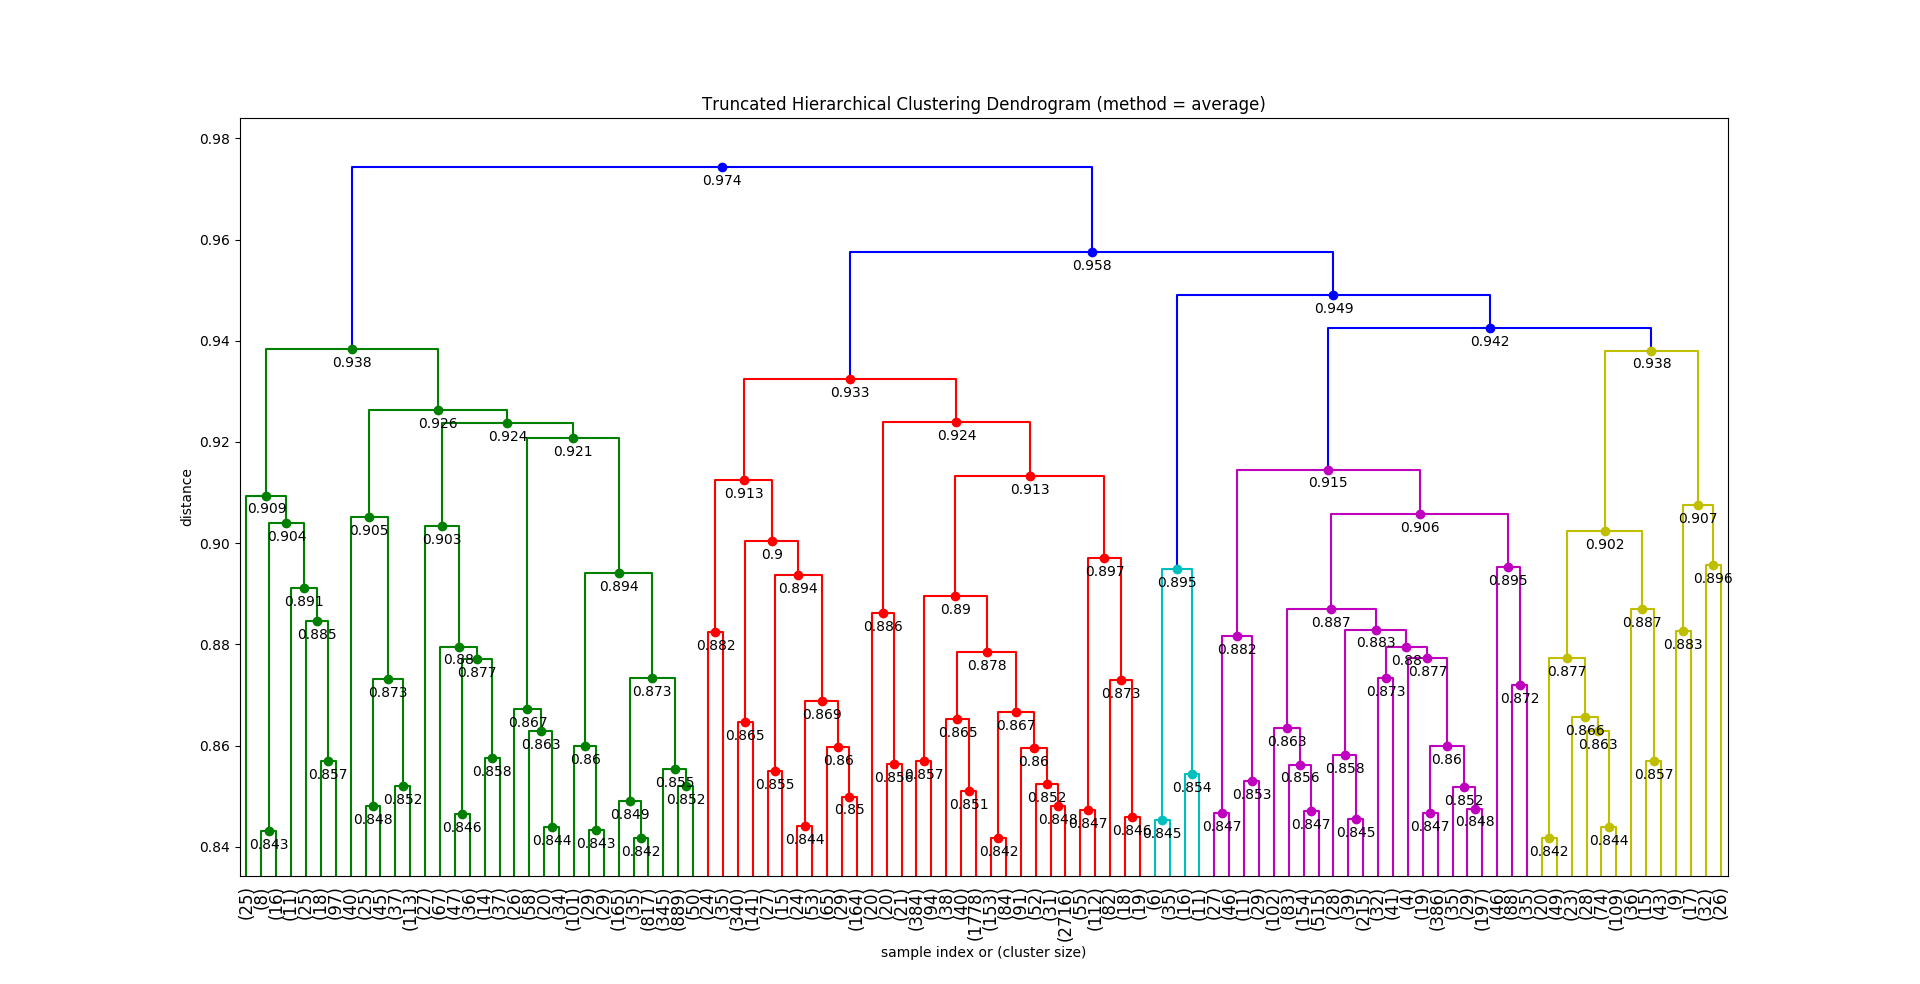
\includegraphics[width=1\textwidth]{images/hierarchical_clustering.png}
    \caption{\textlatin{Hierarchical clustering}}
\end{figure}
\subsection{\textlatin{Distribution based clustering}}
Το \textlatin{Distribution based clustering} είναι μια υποκατηγορία του \textlatin{Hierarchical clustering} και χρησιμοποιείται στις περιπτώσεις που τα δεδομένα έχουν κάποια γνωστή κατανομή όπως
είναι η κανονική ή η Γκαουσιανή. Το \textlatin{Distribution based clustering} μας δίνει τη δυνατότητα να διαχειριστούμε μεγάλα σύνολα δεδομένων και να βρούμε μη γραμμικές σχέσεις ανάμεσα στα
στοιχεία\cite{hcdf}.
